\section{Verification and Validation}

\subsection{Demonstration}

\subsubsection{Complete Decomposition Scenario}
\label{Scenario1}

\begin{figure*}
\centerline{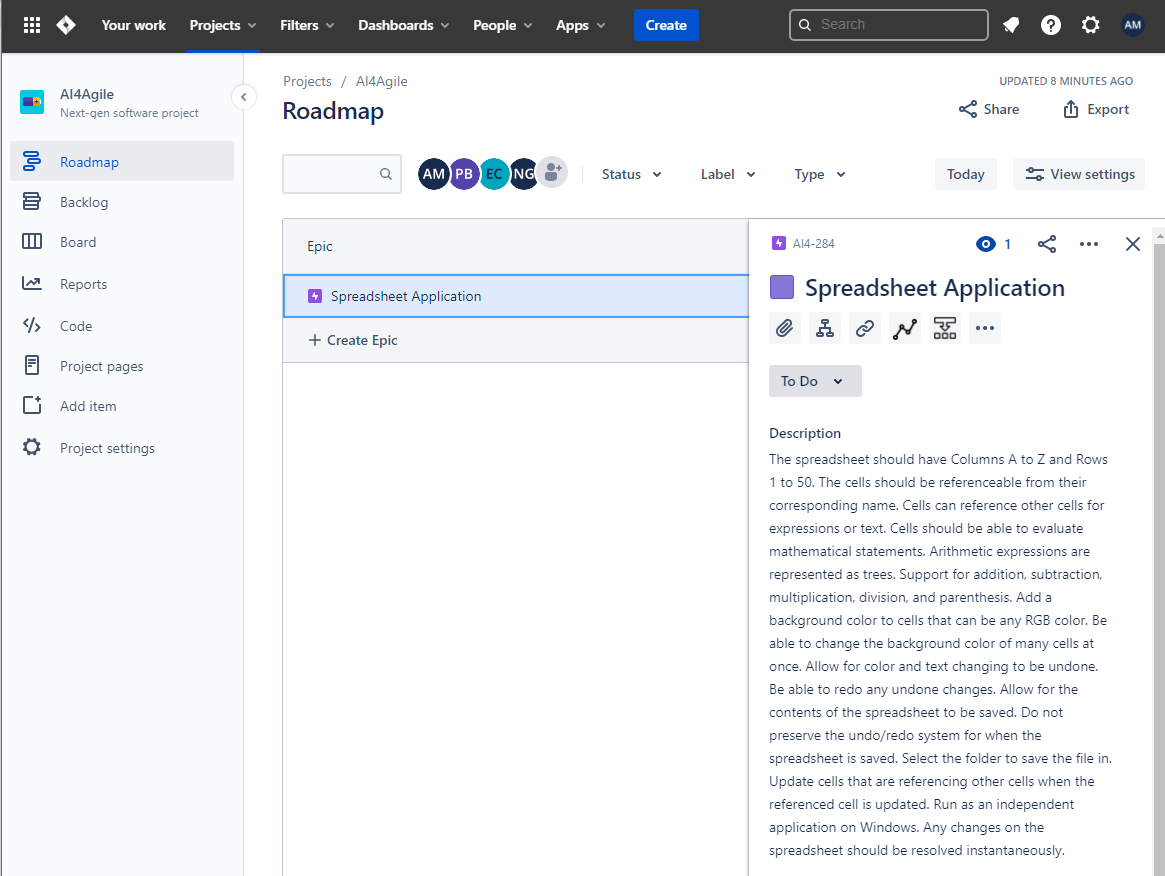
\includegraphics[width=\textwidth,height=\textheight,keepaspectratio]{./figure/Scenario1Figure1.png}}
\caption{Overall view of Jira Roadmap with Decompose Epic button in focus}
\label{fig:Scenario1Figure1}
\end{figure*}

Frank is a software requirements analyst, and he wants to speed up the process of breaking an epic full of requirements into smaller user stories. For this purpose, he installs the AI4Agile plugin to Jira. Frank creates a new epic, puts the requirements for his Spreadsheet Application in as plaintext sentences, and clicks the Decompose Epic button (fig. \ref{fig:Scenario1Figure1}).

\begin{figure}
\centerline{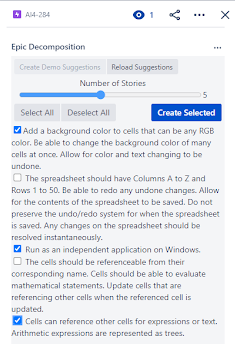
\includegraphics[width=\textwidth,height=\textheight,keepaspectratio]{./figure/Scenario1Figure2.png}}
\caption{View of generated User Story Suggestions}
\label{fig:Scenario1Figure2}
\end{figure}

Now, Frank looks at the suggestions the AI came up with (fig. \ref{fig:Scenario1Figure2}). If he decides he doesn’t like any of these suggestions, he can click the Ignore All button to go back to his Spreadsheet Application epic. If Frank wants more or fewer stories, he can adjust the value on the slider and it will refresh the results. To edit a story, he can click on its text box, then save or cancel those edits. To ignore a story suggestion entirely, he can leave its box unchecked. Once Frank is happy with his resulting user story or the set of stories he wants, he clicks Create Selected. 

After refreshing the webpage, the newly created user stories that Frank approved are visible under the heading of the Spreadsheet Application epic.

If Frank wants to continue the process of breaking up epics, he can go into one of the user stories and click Optimize User Story (fig. \ref{fig:Scenario1Figure3}). Depending on the size of the user story already, it might be broken down into multiple smaller stories, or left alone if it’s already optimized.

\begin{figure}
\centerline{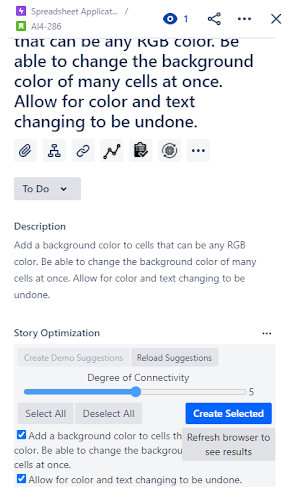
\includegraphics[width=\textwidth,height=\textheight,keepaspectratio]{./figure/Scenario1Figure3.png}}
\caption{User Story Optimization Suggestions page}
\label{fig:Scenario1Figure3}
\end{figure}

Once the Story Optimization Suggestions are generated, Frank has the same options as with the previous stories: to select or deselect stories via the checkboxes, make edits, or ignore all suggestions. In addition to those options, Frank can choose to adjust the connectivity slider to change how closely related items need to be in order to stay with the same story.  

Now there are five user stories, since Story 4 was optimized into two separate stories. To continue the decomposition process, Frank opens a story and clicks Generate Tasks (fig. \ref{fig:Scenario1Figure2}).

\begin{figure*}
\centerline{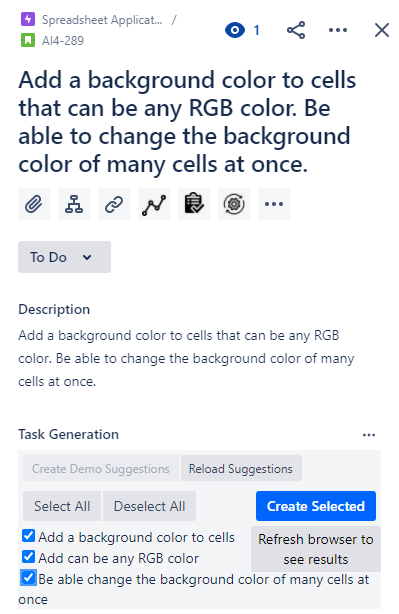
\includegraphics[width=\textwidth,height=\textheight,keepaspectratio]{./figure/Scenario1Figure4.png}}
\caption{Task Suggestions page}
\label{fig:Scenario1Figure4}
\end{figure*}

As before, the options include selecting or deselecting individual suggestions, editing, and ignoring all suggestions. Once he’s happy with the tasks, he clicks Create Selected.

\begin{figure*}
\centerline{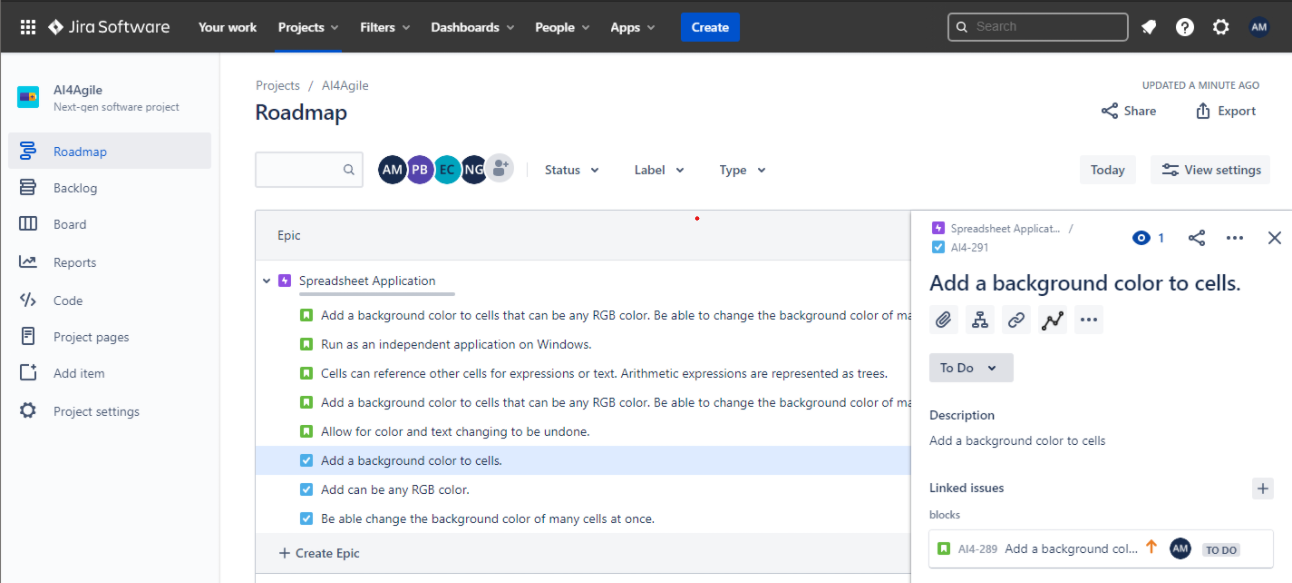
\includegraphics[width=\textwidth,height=\textheight,keepaspectratio]{./figure/Scenario1Figure5.png}}
\caption{View of newly created tasks for one fully decomposed user story}
\label{fig:Scenario1Figure5}
\end{figure*}

The tasks have now been created, and linked to their parent story to indicate a blocking relationship. All Frank had to do was make some decisions and maybe edits, and now he’s got one story fully decomposed (fig. \label{fig:Scenario1Figure5}).

\subsubsection{Relationship Visualization Scenario}
\label{Scenario2}

\begin{figure*}
\centerline{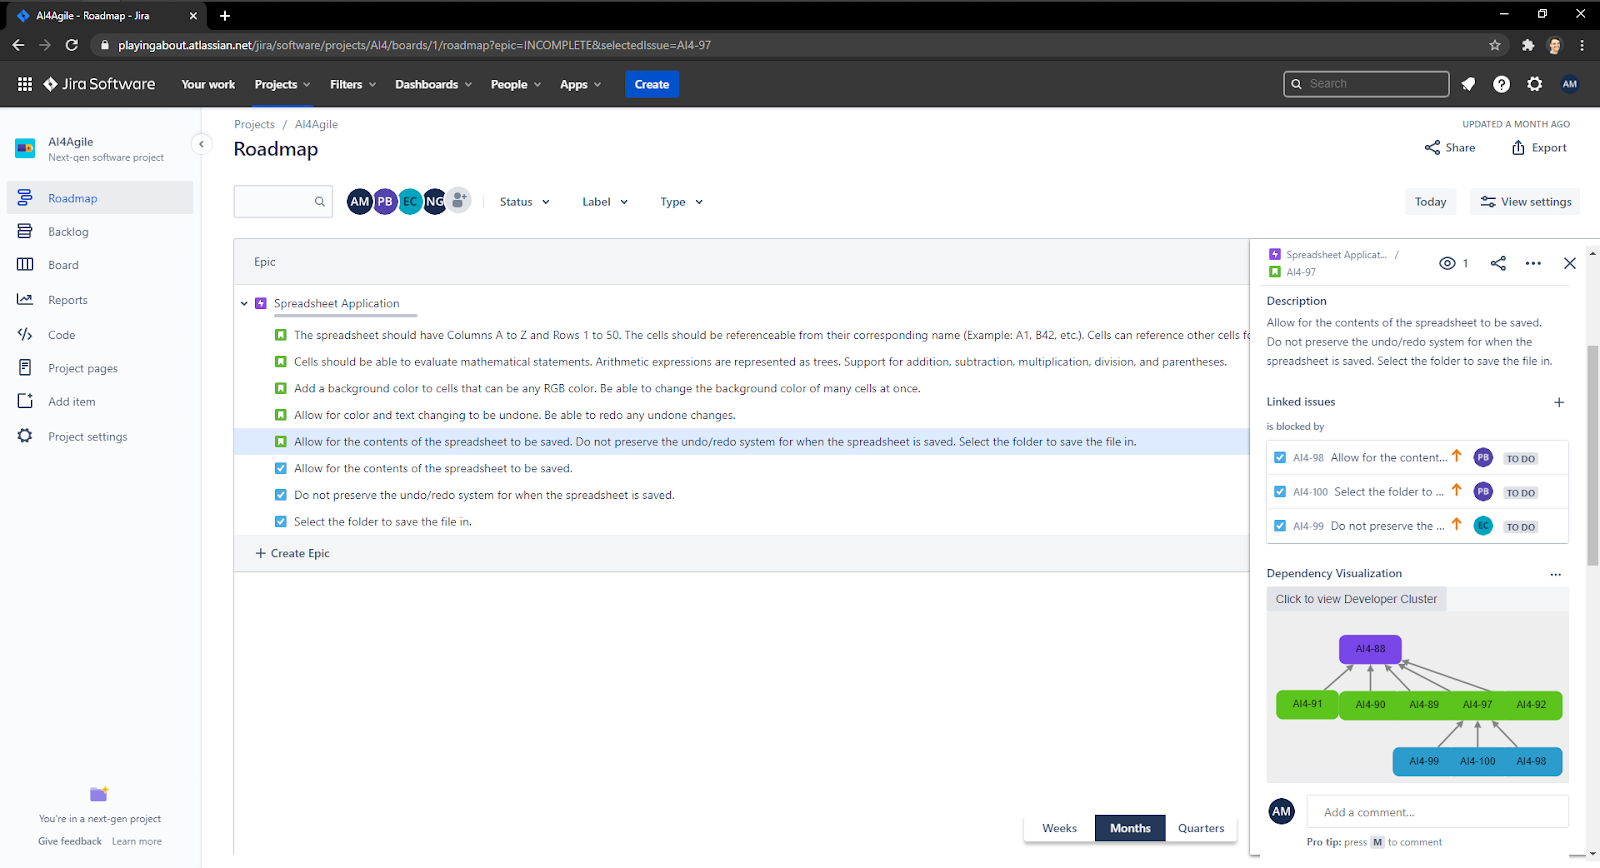
\includegraphics[width=\textwidth,height=\textheight,keepaspectratio]{./figure/Scenario2Figure1.png}}
\caption{A zoomed out view of navigating to the issue relationship graph}
\label{fig:Scenario2Figure1}
\end{figure*}

Madison is a scrum master, and she wants to take a closer look at some of the tasks to make sure the developer assignments make sense. To do this, she uses the AI4Agile Issue Relationship Graph feature by navigating to a certain epic, user story, or task, and finding the graph portion (fig. \ref{fig:Scenario2Figure1}). Now, Madison can see all the available relationships between the task she has selected and other tasks, stories, and the epic they came from. She is better able to decide whether the team members she assigned to these pieces make sense given the relations between them.

\begin{figure*}
\centerline{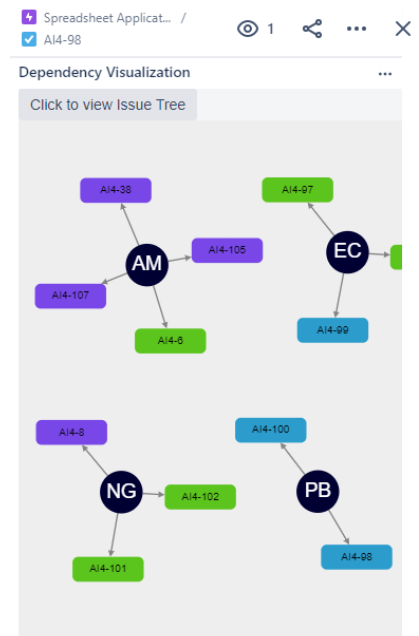
\includegraphics[width=\textwidth,height=\textheight,keepaspectratio]{./figure/Scenario2Figure2.png}}
\caption{Developer cluster graph on a selected task}
\label{fig:Scenario2Figure2}
\end{figure*}

For an alternate view of the relationships, Madison can use the Click to view Developer Cluster button (fig. \ref{fig:Scenario2Figure1}) to see what the current assignments and workload look like for her team (fig. \ref{fig:Scenario2Figure2}). If she wants to go back to the previous graph view, the Click to view Issue Tree button is in the top left corner.